%%____________________________________________________________________________||
\section{Physics objects}
\label{sec:objects}
The definitions of the physics objects used in this analysis follow the ongoing recommendations of the various Physics Object Groups (POGs). 

\subsection{Jets}
\label{sec:jetreco}
Jets are defined as sets of particle-flow (PF) candidates clustered by the
anti-$k_{T}$ jet clustering algorithm \cite{Cacciari:2008gp} with a distance parameter of 0.4
(PFJets). Charged Hadron Subtraction (CHS) is applied, i.e., charged
hadrons that can be traced back to pileup vertices are not clustered.
The four-momenta of jets are initially defined as the four-vector sum of
the four-momenta of the constituent particle-flow candidates and then
scaled by the jet energy correction factors designated as L1FastJet,
L2Relative, and L3Absolute \cite{Chatrchyan:2011ds}.

It should be noted that the early L1 FastJet corrections require
improvements at this stage, and as a result can impact the L2 and L3
corrections. The ``loose'' working point Jet-Id selection criteria was
chosen.

\subsection{b-tagged jets}
\label{sec:btags}
Jets originating from bottom quarks are identified through vertices that are displaced with respect to the primary interaction \cite{Chatrchyan:2012jua}. The algorithm used to tag b-jets is the Combined Secondary Vertex tagger V2, using the ``medium'' working point, which is achieved by requiring a cut of $>$ 0.89 on the algorithm discriminator variable. 
This results in a gluon/light-quark mis-tag rate of $\sim$1 \% (where ``light'' means $u$, $d$ and $s$ quarks) with a b-tag signal efficiency of about 80 \%. 


\subsection{Muons}
\label{sec:muon-id}
Muons are identified according to the ``medium'' working point definition of the recommended identification algorithm, which provides $\sim$ 98 $\%$ efficiency. 
Muons are also required to be well isolated, i.e. with a low activity in the vicinity of their track. 

In the hadronic signal region, a PF-based relative isolation is used with a variable cone size, which is referred to as ``mini-isolation''. 
This isolation algorithm helps in recovering some efficiency in the lepton selection for boosted topology of top quark decays, 
in which the muon's track may be found close to the jet activity due to the boost of the parent top. 
Therefore, the cone size used for the calculation of the lepton isolation is reduced as a function of 
the lepton \Pt, as follows: $R=0.2$ for $\Pt_{\ell}\leq50\gev$, $0.05<R<0.2$ for $50 \gev < \Pt_{\ell} < 200\gev$ and $R=0.05$ for $\Pt_{\ell} > 200 \gev$.

In the \mj and \mmj samples, to have better QCD background control, the standard PF-based relative isolation is used, with a cone size of 0.4.

The transverse momenta of PF neutral and charged candidates within a cone around the lepton are summed. 
The relative combined isolation $I^{rel}_{comb}$ is then defined as 
the ratio of this scalar sum to the transverse momentum of the lepton candidate. 
The neutral hadron and photon contribution to the isolation is corrected 
by subtracting the expected neutral contribution from PU collisions, $\Delta\beta=1/2\sum_{\mathrm{PU}}^{\mathrm{ch had}}{\pt}$. 
The factor 1/2 takes into account the neutral to charged ratio as measured in \cite{CMS-PFT-10-002}. 

Muons are defined as isolated when they have $I^{mini}_{Iso} < 0.2$ within $R$ for mini-isolation, and $I^{rel}_{comb} < 0.12$ .

% Figures \ref{fig:SMStack} and \ref{fig:DMStack} show the relative combined isolation $I^{rel}_{comb}$ for $\mu +$ jets and $\mu\mu +$ jets control sample. The distributions have been weighted according to the cross-section of the respective samples in each region, and an integrated luminosity of 1 fb$^{-1}$ at $\sqrt{s}$ = 13 TeV. Isolated muons promptly produced in the decays of W and Z bosons dominate the region $I^{rel}_{comb}$ $<$ 0.12.

Muons are vetoed in the definition of the hadronic signal region, 
as described in Section \ref{sec:preSelection}, while 
control regions with one muon (``\mj'') or two muons (``\mmj'') are defined for the purpose of the background estimation, 
as described in Section \ref{subsec:mucontrolSelection}.

% now we're using mini isolation this is no longer relevant:

% \begin{figure}[h]
%   \centering
%   \subfigure[Relative combined isolation variable for \texorpdfstring{\mj}{muon plus jets}
%   control sample]{
%     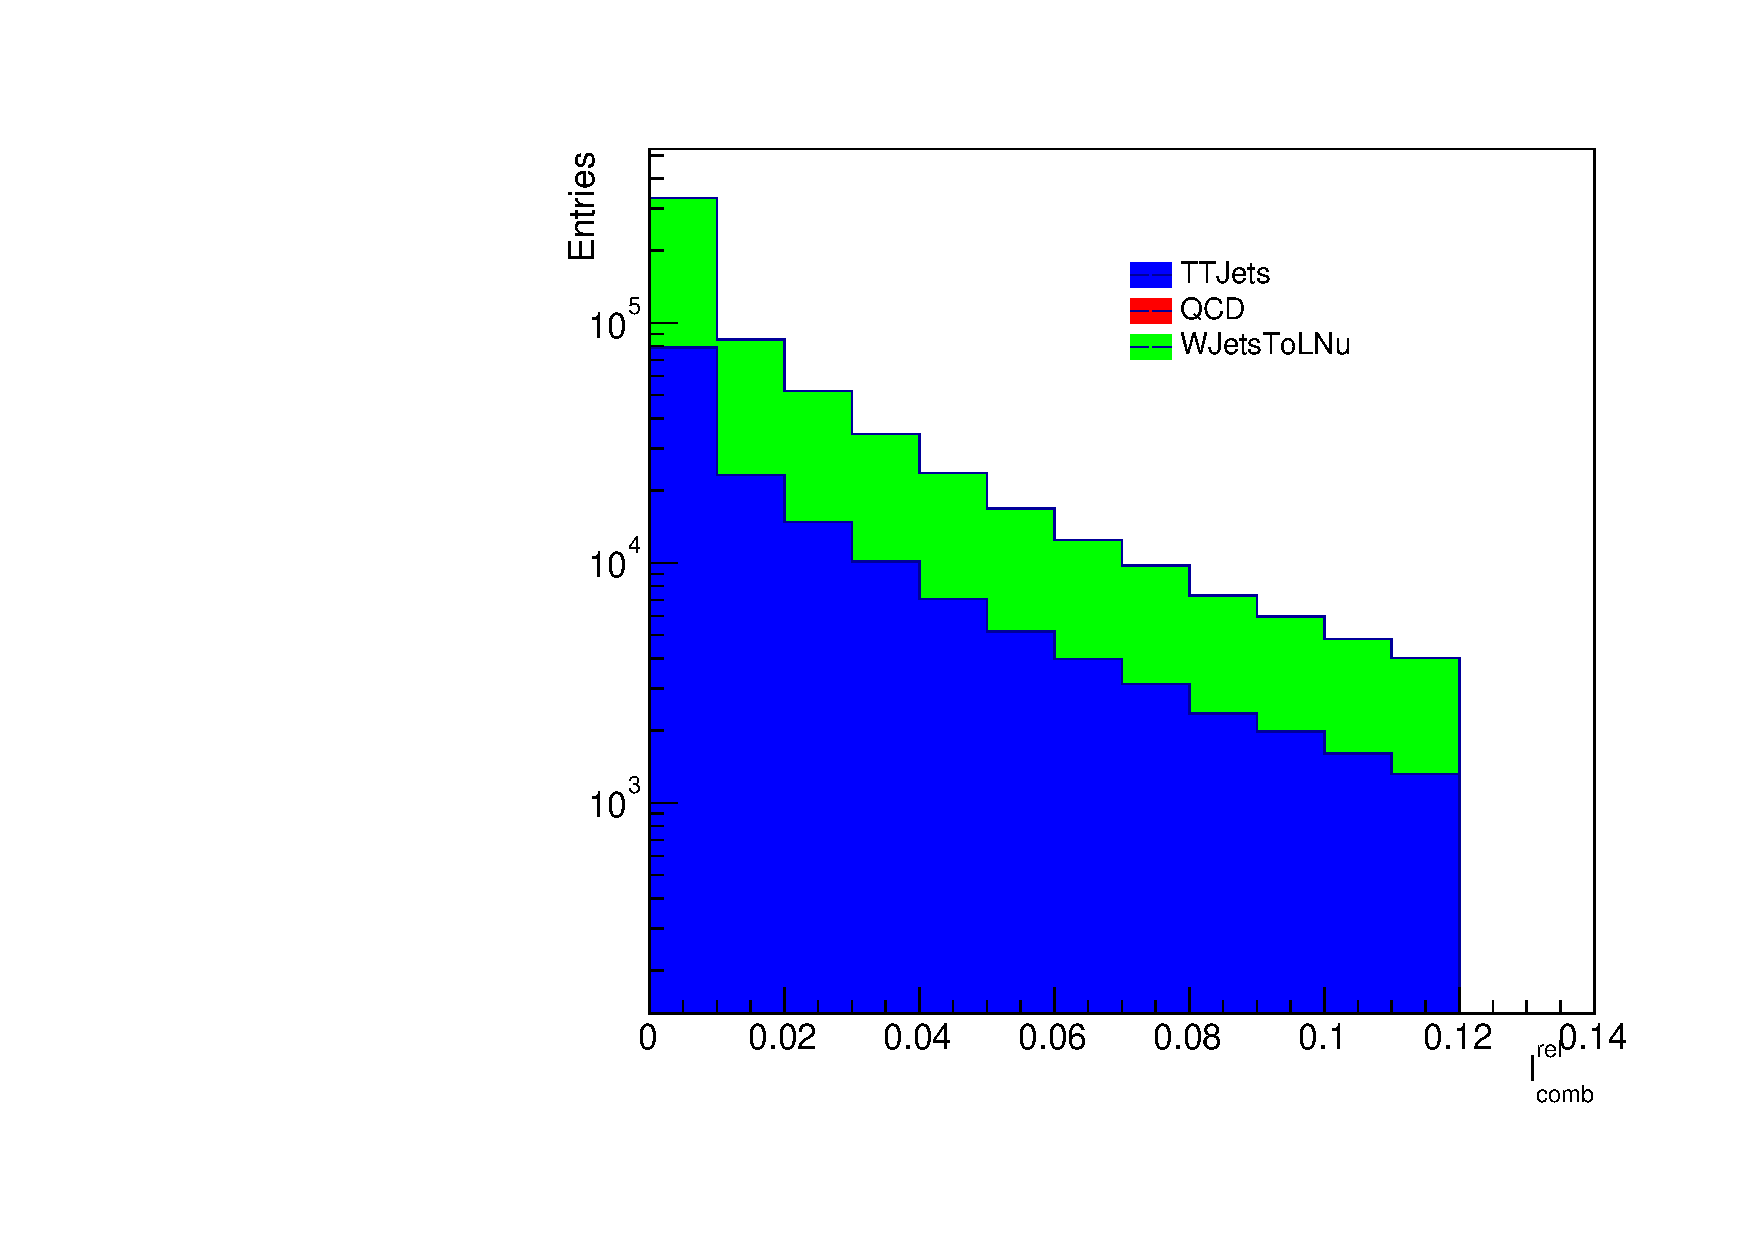
\includegraphics[width=0.5\textwidth]{figures/PhysicsObjectsPlots/SingleMuStack.pdf}
%     \label{fig:SMStack}
%   }~~
%   \subfigure[Relative combined isolation variable for \texorpdfstring{\mmj}{di-muon plus jets}
%     control sample]{
%     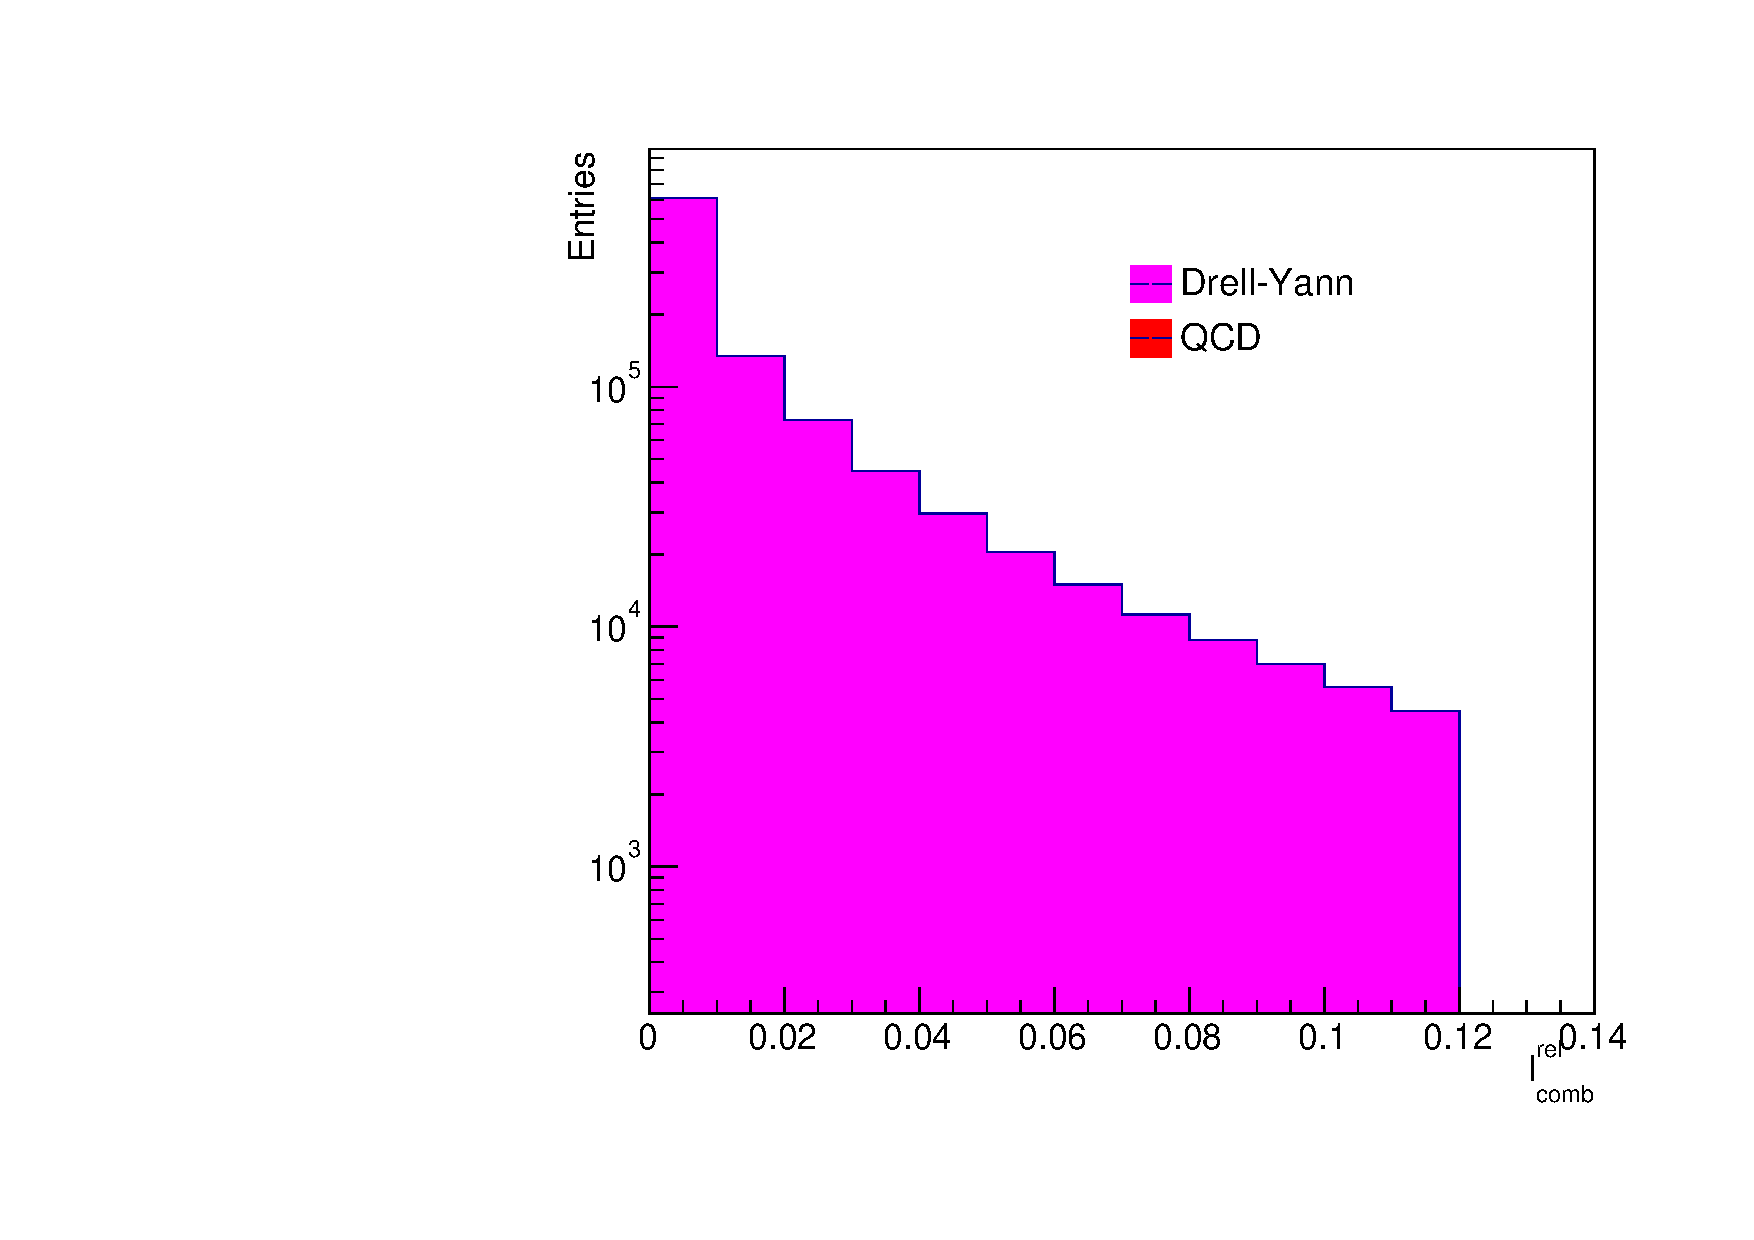
\includegraphics[width=0.5\textwidth]{figures/PhysicsObjectsPlots/DoubleMuStack.pdf}
%     \label{fig:DMStack}
%   }~~  
% \caption{$I_{comb}^{rel}$ for \texorpdfstring{\mj}{muon plus jets} & \texorpdfstring{\mmj}{di-muon plus jets} control samples}
% \end{figure}


\subsection{Photons}
\label{sec:photon-id}
Photons are identified according to the ``tight'' working point definition ($\sim$ 71 $\%$ efficiency) 
of the simple cut-based photon identification algorithm \cite{photon-id} 
and required to be well isolated. 
A PF-based isolation is used with a cone size $\Delta R$ $<$ 0.3 and $\rho$ x $A_{eff}$ corrections are applied to remove the effects of pileup \cite{pf-photon}. 
Table \ref{tab:photon-id-gamma} summarises the identification and isolation selection used. 

Photons are vetoed in the definition of the hadronic signal region, 
as described in Section \ref{sec:preSelection}, while a 
control region with one photon (``\gj'') is defined for the purpose of the background estimation, 
as described in Section \ref{subsec:photoncontrolSelection}.


\begin{table}[ht!]
  \caption{Photon identification (``tight'' working point).\label{tab:photon-id-gamma}}
  \centering
  \footnotesize
  \begin{tabular}{ ccc }
    \hline
    \hline
    Categories                    & Barrel                             & EndCap                             \\
    \hline
    Conversion safe electron veto & Yes                                & Yes                                \\
    Single Tower H/E              & 0.05                               & 0.05                               \\
    $\sigma_{i\eta i\eta}$        & 0.01                               & 0.0267                               \\
    PF charged hadron isolation   & 0.91                               & 0.65                               \\
    PF neutral hadron isolation   & 0.33 + $ e^{0.0044 \times \pt^{\gamma} + 0.5809}$  &  0.93 + $ e^{0.0040 \times \pt^{\gamma} + 0.9402}$ \\
    PF photon isolation           & 0.61 + 0.0043 $\times$ $\pt^{\gamma}$ & 0.54 + 0.0041 $\times$ $\pt^{\gamma}$ \\
    \hline
    \hline
  \end{tabular}
  \end{table}


\subsection{Electrons}
\label{sec:electron-id}
Electrons are identified according to the ``loose'' working point definition ($\sim$ 90 $\%$ efficiency) 
of the cut-based identification \cite{electron-id} for the purpose of the electron veto in the signal region, while the ``tight'' working point ($\sim$ 70 $\%$ efficiency) is used for the selection of electron in the corresponding control regions. 

Electrons are also require required to be well isolated. 
Similar to muons, in the hadronic signal regions, a PF-based isolation \cite{pf-photon} is used with a cone size determined by the mini isolation algorithm (see Sec.~\ref{sec:muon-id}) and $\Delta \beta$ corrections are applied to remove the effects of pileup, while in \ej and \eej control regions, a PF-based isolation with a fixed cone size of 0.4 is used.
Table \ref{tab:ele-id} summarises the identification and isolation selection used for the PHYS14 exercise. In the future it is intended to move to a $\rho$ x $A_{eff}$ pileup correction method as recommended by the electron POG.

Electrons are vetoed in the definition of the hadronic signal region, 
as described in Section \ref{sec:preSelection}, while 
control regions with one electron (``\ej'') or two electrons (``\eej'') are defined for the purpose of the background estimation, 
as described in Sections \ref{subsec:elecontrolSelection} and \ref{subsec:dielecontrolSelection}.


\begin{table}[h!]
  \caption{Electron identification (``tight'' working point).\label{tab:ele-id}}
  \centering
  \footnotesize
  \begin{tabular}{ lcc }
    \hline
    \hline
    Categories                                               & Barrel    & EndCap    \\
    \hline
    $\Delta \eta_{In}$                                       & 0.00926   & 0.00724  \\
    $\Delta \phi_{In}$                                       & 0.0336    & 0.0918  \\
    $\sigma_{i\eta i\eta}$                                   & 0.0101    & 0.0279  \\
    H/E                                                      & 0.0597    & 0.0615   \\
    d0 (vtx)                                                 & 0.0111    & 0.0351  \\
    dZ (vtx)                                                 & 0.0466    & 0.417  \\
    $\lvert(1/E_{\textrm{ECAL}} - 1/p_{\textrm{trk}})\rvert$ & 0.012     & 0.00999  \\
    Mini-Iso PF relative isolation                           & 0.1       & 0.1       \\
    Rel-Iso PF relative isolation                            & 0.0354    & 0.0646       \\
    Missing hits                                             & 2         & 1         \\
    \hline
    \hline
  \end{tabular}
  \end{table}


\subsection{Single isolated tracks}
\label{sec:SIT}

A single isolated track (SIT) can be used to identify W bosons through their leptonic decays: 
W $\rightarrow$ $\mu \nu$, W $\rightarrow$ $e\nu$, and W $\rightarrow$ $\tau$($\rightarrow l$) $\nu$. 
Single prong decays of the tau lepton can also be identified: W $\rightarrow$ $\tau$ ($\rightarrow$ h$^{\pm}$ + n$\pi^{0}$) $\nu$. 
A single isolated track comprises a charged PF candidate with $\Pt > 10 \gev$, $\Delta z(\mathrm{track}, \mathrm{PV}) < 0.05 \, \mathrm{cm}$ 
and with a relative isolation smaller than 0.1, where the isolation is determined from the sum 
of the \Pt of the charged PF candidates within $\Delta R < 0.3$.

SIT are vetoed in the definition of the hadronic signal region, 
as described in Section \ref{sec:preSelection}.

%% % No more needed
%% \begin{table}[h!]
%%   \caption{Single isolated track identification.\label{tab:sit-id}}
%%   \centering
%%   \footnotesize
%%   \begin{tabular}{ lc }
%%     \hline
%%     \hline
%%     Track \Pt                      & $>10\gev$  \\
%%     $\Delta z (\textrm{track,PV})$ & $<0.05\cm$ \\
%%     Charge                         & $\neq 0$   \\
%%     Relative track isolation       & $<0.1$     \\
%%     \hline
%%     \hline
%%   \end{tabular}
%%   \end{table}

\subsection{Missing transverse momentum}
Missing transverse momentum (\met) is defined as the opposite of the vector sum
of the transverse momentum of all particle-flow candidates in the event.
The Type-I \met correction \cite{Khachatryan:2014gga} is applied, i.e., the transverse momentum of
the particle-flow candidates clustered as jets are replaced with the
transverse momentum of the jets that are scaled by the jet energy
correction factors.

The \met is used in the definition of 
the transverse mass, $M_{T}$, which is in turn used as part of
the selection criteria that define the single muon control sample 
(section \ref{subsec:mucontrolSelection}), and to define a cleaning filter applied after the
$\alpha_{T}$ requirement, as described in Section \ref{sec:selection}.



%%____________________________________________________________________________||
